\section{UPPAAL Model Implementation}

\subsection{Priorities and design decisions}

The problem of modeling an algorithm requires first identifyung those aspects of the algorithm that are of relevant for verification, and then simplifying and abstracting as much as possible while representing those interesting aspects faithfully.

In our case, considering the research questions, we are interested in the global state of the network, specifically the notion of iterations as a measure of running time.

We also considered different levels off abstraction in modeling, in part to explore the possibilities and limitations of modeling using probabilistic timed automata.

Finally, we prioritized respecting the constraints of the algorithm, specifically that robots should only have local information. We examined whether the process of transmitting local knowledge across the graph would introduce subtle changes to the theoretical behavior of the algorithm.
As we did not have a concrete implementation of the algorithm, we were interested in how much of a challenge it was to respect these constraints.

As a result the model represents a quite faithful simulation of the robots interactions as described in the paper. However, this required us to make a few implementation decisions of note that were left under-specified by the original authors.

This design decision introduced additional steps in the modeling process, as it requires modeling a communication algorithm, which in turn required additional debugging, implementation and verification steps.

As we are interested in the state of the network as a whole, we abstract away the concrete communication between robots. Instead, we simulate communication limits using a mask for each robot over global arrays indexed by the id of each robot. This mask is called \texttt{C}, and determines the network by describing local connection group for each robot. Following is an example og how a network of three robots in a line would look like:

\begin{verbatim}
bool C[3][3] = {{false, true, false},
                {true, false, true},
                {false, true, false}}
\end{verbatim}

This means that all information that a robot may request of a neighbor is available to be read without modeling concrete communication between those robots.

\subsection{Overview of model}

In our model, each robot is a process with an ID and five possible locations, including an initial and a terminal location.

The network can have either a completely random distribution of initial preferences, or it can be random with a number of seeded robots.
The number of seeded robots are controlled with the constant \texttt{SEEDNUM}, and the robots with a smaller id value get 100\% preference towards choice 0. This corresponds to Lie \& Lee's use of seed robots (section 3.4).
Though they do not specify the exact preference distribution given to seed robots, our results match theirs (see results section).

At location \texttt{PreferencesUpdated}, the robot has updated their preferences and their exhibited decision. At location \texttt{FindingDecisionGroup}, the robot is in the process of determining its consensus group $D$. At location \texttt{AwaitingNeighbors} the robot either terminates (if a global consensus has been found) or it moves on to a new iteration of updating its preferences (by traversing the edge to \texttt{PreferencesUpdated}).

\begin{figure}[H]
    \centering
    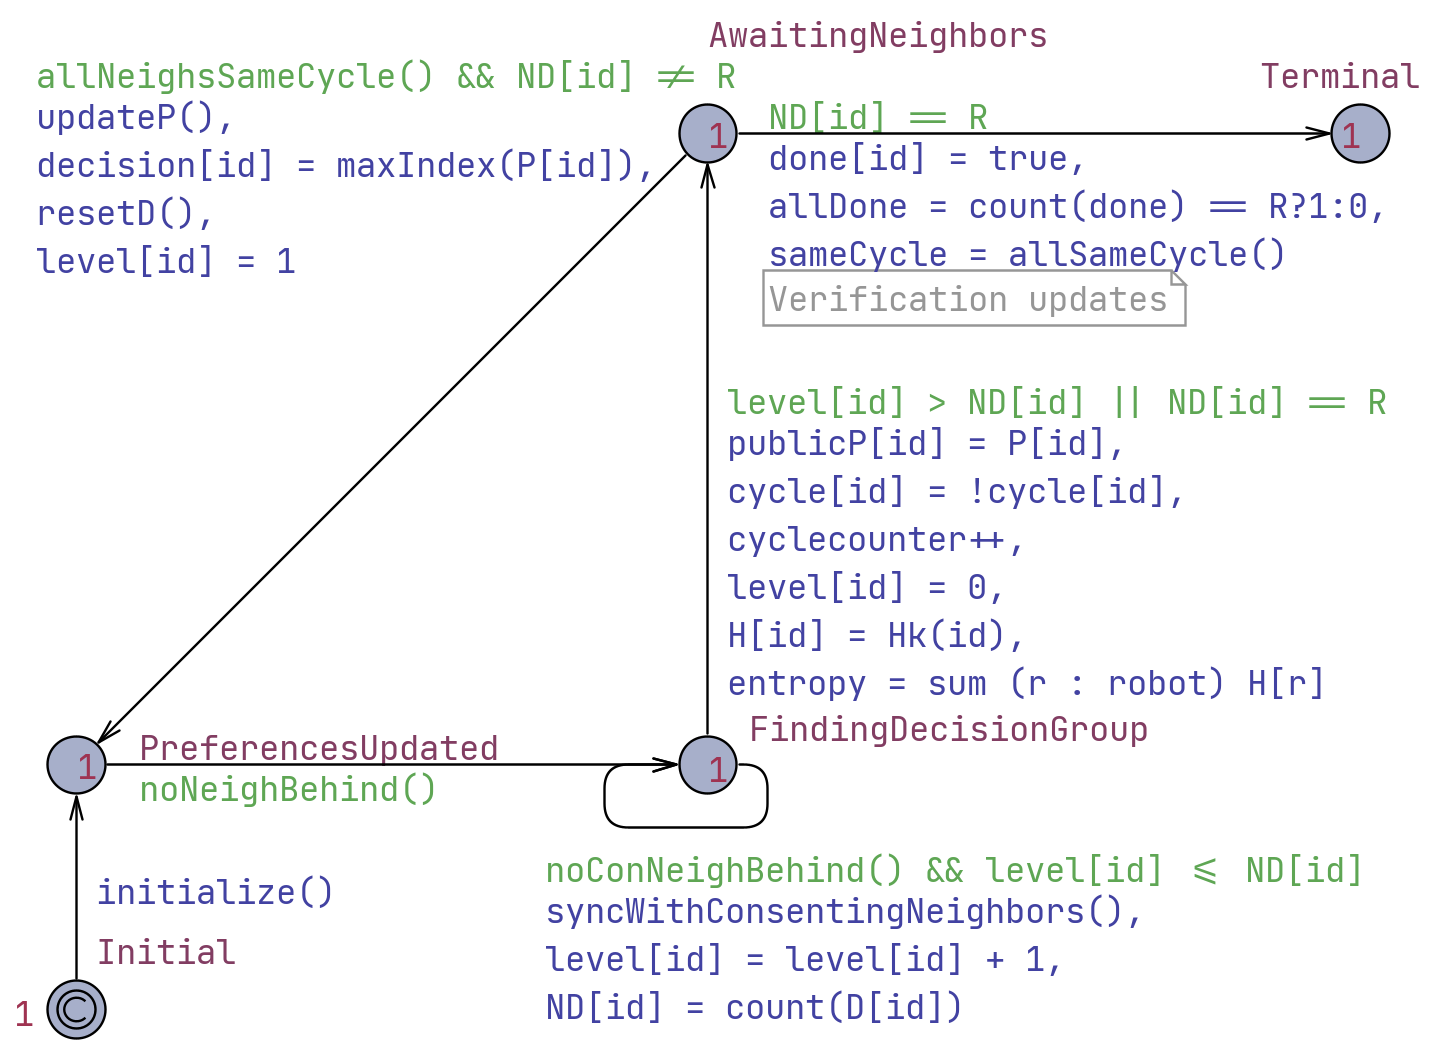
\includegraphics[width=\linewidth]{pictures/Model screenshot 2025-05-11.png}
    \caption{The Robot template in UPPAAL. Besides variable and function declarations, the system consists of $m$ instantiations of this state machine unique id values. Each state is named (in brown, capitalized), and has a rate of exponential of 1. Each edge transition has a guard statement (boolean expression) and a comma-separated sequence of assignments and method calls. Guard statements are in green and appear above assignments. They are placed as a block close to the edge they guard.}
    \label{fig:model}
\end{figure}

The edge from \texttt{Initial} to \texttt{PreferencesUpdated} directly corresponds to the initialization of the algorithm (section 2.1).
The edge from \texttt{AwaitingNeighbors} to \texttt{PreferencesUpdated} corresponds to both (section 2.2) preference updating via local interaction and (section 2.3) internal processing for decision uncertainty reduction.

All the edges leading to or originating in \texttt{FindingDecisionGroup} are needed to update the robots' local understanding of their consensus group, which is not specified as a separate step in the algorithm, but which requires a separate step in the model to preserve the constraint of local communication. We describe the algorithm for calculating consensus groups below.

\begin{table}
\begin{center}
\begin{tabular}{ lll } 
\hline
Code & Algorithm & Meaning \\
\hline
\texttt{D[id]} & $D_k$ & Consensus group for robot \texttt{id} / $k$\\ 
neighbors, or \texttt{C[id]} & $C_k$ & The connection group for robot \texttt{id} / $k$\\ 
\texttt{ND[id]} & $N_k$ & Size of consensus group for robot \texttt{id} / $k$\\ 
\texttt{P[id][j]} & $P_k(j)$ & Robot \texttt{id} / $k$'s preference toward decision $j$ \\
\texttt{decision[id]} & exhibited decision & The highest preference value of robot \texttt{id} \\
\texttt{R} & $m$ & Number of robots in system. \\
\texttt{Q} & $n$ & Number of decisions \\
cycle & iteration & A full update of preferences. \\
\texttt{EMPIRICAL} & $\lambda_T$ & The empirical threshold value convergence\\
\texttt{s[j]} & $s(j)$ & The rank of choice j for a given robot.\\
\texttt{Hk()} & $H_k$ & (section 3.1) Entropy value for robot $k$\\
\texttt{entropy} & $\sum H_k $ & Total entropy of system\\
\texttt{updateP()} & $P_k$ & Eq. 1. Include uncertainty reduction if relevant. \\
\texttt{divergence()} & $\lambda_k$ & Eq. 2. The degree of divergence for robot k\\
\texttt{accConvergence()} & $P^{new}_k$ & Eq. 3. The method normalizes the new values.\\
\texttt{L(s[j], Ll, Lu)} & $\mathscr{L}(s(j))$ & Eq. 4. The linear multiplier for choice $j$.\\
\hline
\end{tabular}
\caption{Explanation and translation of coding variables to algorithm terminology}
\label{tab:gloss}
\end{center}
\end{table}

\subsubsection{Timing and synchronization}

Because the paper did not specify any absolute or relative timing requirements, we decided not to give time invariants to locations, and rather uniformly give each location an exponential rate of 1. In our system, then, time is a proxy for the average number of edge traversals of the robots.

In terms of synchronization, the robot uses three local variables: the booleans \texttt{mayContinue} and \texttt{cycle[id]} and an integer \texttt{level[id]} bounded by the number of robots \texttt{R}.

\texttt{mayContinue} guards most edge traversals and is a product of the other sunchronization variables, depending on robot's current location.

\texttt{cycle[id]} represents the current cycle of the robot, relative to its neighbors. The cycle is flipped when traversing the edge between \texttt{FindingDecisionGroup} and \texttt{AwaitingNeighbors}. To continue from that location, all of a robots neighbors must be on the same cycle. Deadlocks are avoided because no robot will traverse a full cycle before all of its neighbors has exited \texttt{AwaitingNeighbors}, as they also have to synchronize at location \texttt{PreferencesUpdated}.

\texttt{level[id]} represents the progression of the robot within its current cycle, and is reset to 0 with each new cycle. Level 1 and above signifies that a robot has updated its preferences and exhibited decision. By waiting for all its neighbors to reach level 1 a robot ensures that it knows which neighbors exhibits the same decision (consents with) it, which is a precondition to determine its consensus group. 

When determining the consensus group, a robot continuously updates its consensus group to be the union of all its neighbors. This process is synchronized using levels, such that all information is guaranteed to travel throughout the consensus group withing \texttt{R} levels. We give a more thorough walkthrough of this algorithm below.

In total, local synchronization is quite strict, a robot waits for all its neighbors to reach a certain state twice within each cycle, and potentially waits for all consenting neighbors at each level between 1 and \texttt{R}. However, at a global level, we this model makes no assumptions about neither speed or interleaving of updates. There is no assumed global clock, and in a large network, at a given time before consensus is reached, robots may have completed quite different numbers of cycles, while in the end they will all have completed an equal number of cycles. 
This is interesting for two reasons: The loose global synchronization shows that the properties we test hold for networks without global coordination, and the strict local synchronization is part of the networks strategy to increase fairness.

\subsubsection{Fairness and atomic updates}

When considering the implicit assumption in the original article that robots are globally synchronized in iterations, we find that the specific synchronization policy influences the behavior of the algorithm.
A robot that reevaluates their preferences at a higher rate than its neighbors becomes more influenced by its neighbors than in reverse. Also, robots out of sync introduce possibilities of data consistency errors as robots request and update their preferences, and determine their consensus groups concurrently.
One way of solving this would be to have global synchronization with a predetermined order of updates for all robots, however as noted above, we were interested in respecting the requirement that robots do not communicate globally.

By using the above synchronization methods, we ensure that all robots complete the same number of preference updates, and that at any given time, a robot can at most be one update ahead or behind its neighbor. With no further modification, we would be left with the problem that the result of updating a robots preferences is influenced by the sequencing of when the robots in its connection group update their preferences.

We solve this by implementing a public / private distinction for the preferences. A robot updates its \texttt{P[id]} array by reading from each robot $r$ of its neighbors'  \texttt{publicP[r]} array. The  \texttt{publicP} arrays are updated when entering the \texttt{AwaitingNeighbors} location. In this way the updates to a robot and its neighbors preferences occur as if instantaneously from the perspective of a given robot.

\subsection{Algorithm for locally determining consensus group}

Since any change in exhibited decision in any robot can result in a drastic change in the consensus group of another robot, we consider the most transparent and faithful model to be one in which every robot recalculates its consensus group at each cycle.

The algorithm has three requirements: The consensus groups should be correct, it should not change the behavior of the algorithm and it should only use local information. Further, we want the process to not take too much time, and it should be as simple as possible so it is easy to analyze and reason about.

In our approach, each robot starts out by including only themselves in their decision group. Then all robots continuously pull decision group information from their connected consenting neighbors, and eventually, all robots will be aware of all members of their consensus group.

To synchronize this behavior, a robot is only allowed to pull information if no consenting neighbor is at a lower level than it. When it has pulled information, it increments its level and recalculates its local understanding of its consensus group size.
This ensures that all information will be travel across the consensus group. 
In the worst case, the information from one robot travels in a path including all other robots in the consensus group before reaching a final robot, and so the total number of levels gained required to be certain that all information has been gained is equal to the number of robots in the correct consensus group.
Because of this insight, we can reason that if a robots has a local understanding of its consensus group size $d$, and it has gained $d$ levels, then it is certain that it has found the correct consensus group.

An inductive reasoning of the above arguments goes as such: 

In the base case, where the correct $|D| = 1$, a robot initially believes $|localD| = 1$, which is correct. However, to be certain it is correct, the robot tries to pull information from its neighbors, does not find any new information, gains a level, and concludes that it is finished, since it has gained 1 level and has $|localD| = 1$. If $|D| = 2$, the robot must have found that out when asking its consenting neighbor, just as the consenting neighbor must have found that out when asking it. 

If $|D| = 3$, at least one robot must find out about both of its connected consenters in the first level, in which case it repeats for a few levels without learning anything new. If any robots do not find that out in the first level, they still must find one other robot and so have a $|localD| = 2$. In that case, they have still only gained one level so repeat the process once more. They must find out about the final robot in the next level, since they are connected to a robot that has found out about it.

Described another way, if a robot has $|localD| = d$ and is level $d-1$, it must pull information again. Then it either does not find anything new or does, in which case $|localD| = e$, $e > d$ and the robot must continue pulling until it is level $e-1$, at which point the scenario repeats.


\subsection{Verification of model}

While we are using the model to verify properties of the algorithm, we have also separately worked on verifying the quality of our model itself.

We made another model using depth-first search to determine the decision group sizes and simpler synchronization policies. 
The idea is to compare the behavior of those models. (DO WE FIND ANY DIFFERENCE IN BEHAVIOR?)

We have come up several test topologies of small networks. 
These include a minimally connected (a line) and a maximally connected network, a circular network and a randomly generated network.

The basic properties we check to see if the networks behave correctly are:

\begin{enumerate}
    \item All robots terminate in the same cycle and within a bounded time frame.
    \item The model-checker fails to find an example of a network that after a bounded time frame is not completed.
    \item The expected number of cycles and expected time before termination are measured as a sanity check to see if performance changes unexpectedly after changes to the network or to the model.
    \item The entropy is measured to show that entropy falls with a sufficiently high \texttt{empirical} value, and does not if \texttt{empirical} is 0.
    \item The chance of the consensus being decision 0 is measured, to make sure it corresponds to random chance for unseeded networks, and is high for seeded networks.
\end{enumerate}

See \ref{fig:properties} for the concrete syntax.

We have also continuously inspected concrete simulation traces to compare actual behavior with expected behavior.

Finally, we have used a few evaluation variables to construct basic verification queries to check in the statistical model checker.

\begin{figure}[H]
    \centering
    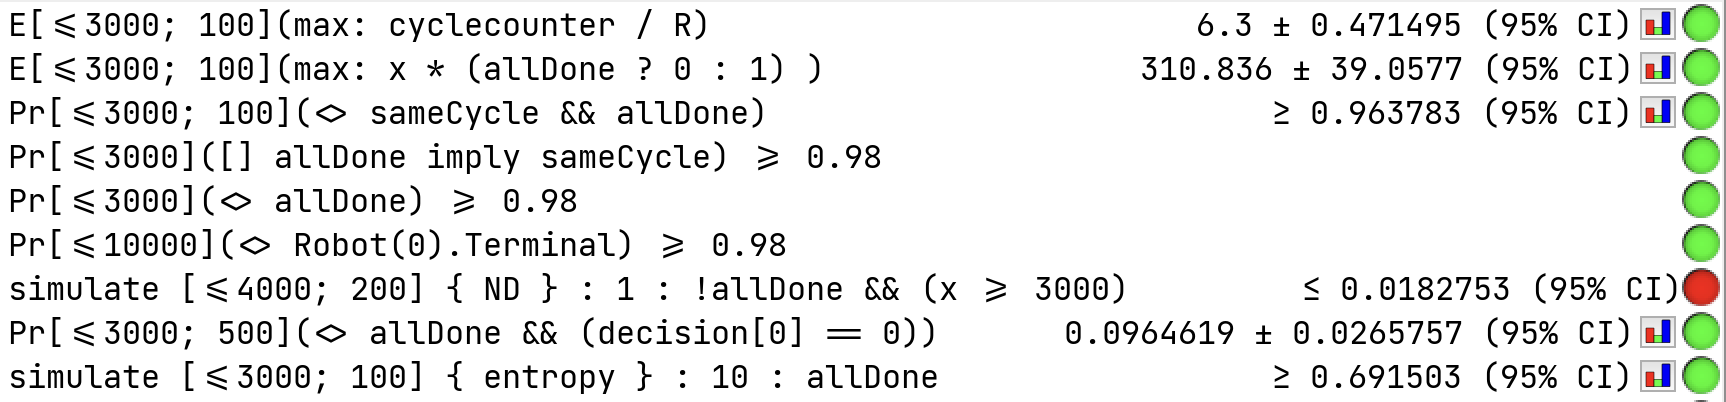
\includegraphics[width=\linewidth]{pictures/Properties.png}
    \caption{All properties checked to verify model.}
    \label{fig:properties}
\end{figure}

\subsubsection{Evaluation variables}

We have introduced five global variables to monitor properties of the algorithm.
\texttt{done[id]} reflects if a robot is in the terminal state. \texttt{allDone} reflects if all robots are in the terminal state. \texttt{sameCycle} reflects if all robots are in the same cycle after termination. \texttt{cyclecounter} counts the total times any robot has completed a cycle. If all robots end in the same cycle, then \texttt{cyclecounter / R} gives the number of (global) cycles before a consensus was reached.
\texttt{H} and \texttt{entropy} are measures of the global entropy in the system, derived using the formula in Liu \& Lee (section 3.2).

\subsubsection{Uncertain quality of convergence acceleration algorithm}

We have implemented the decision uncertainty reduction part of the original algorithm.
It relies on an "empirical threshhold value" (section 2.3) $\lambda_T$.
We took that implicitly to mean that the value should be determined by experiment based on how much of a performance improvement it produces in terms of cycles before a consensus is reached. However, we have not found a clear example of any value resulting in faster consensus times. We have tested with many different values in the range of 0.001 to 100.0, and conversely tend to see increased average cycles to reach consensus. We have even found very rare edge cases where circular topologies can end in a stalemate with two equally large and dominating consensus groups for large values of $\lambda_T$ ($>1$).
We are confused and concerned about this behavior. On the one hand, we may have implemented the algorithm incorrectly. We can of course not prove the absence of bugs, but also, the process itself is not fully specified in the original paper; It is not clear how the resulting values should be normalizes (which they have to by definition of $P_k()$ as a probability mass function), nor is it clear if the convergence acceleration should be added to the preference update process or replace it.

On the other hand, the behavior makes sense intuitively. If a network at some point starts containing multiple locally converged competing clusters (which happens easily in linear or circular topologies), they will become increasingly confident in their decision and so it is to be expected that more cycles will be required for one cluster to convince another.

We therefor also consider if this is intended behavior, because convergence acceleration improves some other metric than number of cycles till consensus. E.g. the authors point out convergence acceleration reduces discrete entropy. We might also consider that the process qualitatively improves results in a way not easily measurable.

This is an area we will continue to explore to find some more satisfactory answers.